\chapter{その他の検討事項}
本節では,データの特徴を考慮して考案したNMFの制約とモデルエビデンスの計算方法を紹介する.

\section{分解能の決定}
ニューロンの活動データの扱いには時間分解能と空間分解能の2つの側面から検討する必要がある.
時間分解能については,蛍光強度データをそのまま用いる,時間窓に区切るなどが考えられる.
空間分解能については,ニューロン1個を見る場合,2個を見る場合,複数を見る場合が考えられる.
手法によってどのレベルでデータを扱うかが異なる.
\Tabref{tab:methods}にカルシウムイメージングデータを解析する際に使えそうな手法を載せる.
これらの手法ではニューロンのネットワーク構造変化やグループの活動の変化などを観察できる.
提案アプローチでは行列分解を使いニューロングループを推定し,グループの活動時系列の情報は使わなかった.
しかし,提案アプローチでも時間窓で区切ってニューロングループの推定を行えばクラスタの変化は抽出できる.
その際,あまりに短い時間窓内では意味のある情報が取り出せない可能性がある.
ニューロングループがどれくらいの頻度で活動するのかをある程度の仮定を置いて時間窓を決定する必要がある.

\begin{table}[htb]
  \center
  \begin{tabular}{|c|cc|} \hline
    & 生データ & 時間窓で区切る \\ \hline
    ペアで見る & 時系列クラスタリング,TE & glasso,類似度+クラスタリング\\
	  複数で見る & 行列分解 & ロジスティック回帰,時系列クラスタリング \\ \hline
  \end{tabular}
  \caption{カルシウムイメージングデータ解析に使えそうな手法}
  \label{tab:methods}
\end{table}

\section{スケール除去}
ニューロンごとに発現している蛍光タンパク質の量や細胞の大きさが異なる.
そのため,ニューロンごとのバイアスが観測データに載っていると考え,バイアスを除去する方法を試した.
この時の数理モデルは以下のようになる:
\begin{equation}
	X = DC + H + B,
\end{equation}
ただし,$B \in \mathbb{R}_+^{I\times J}$は行ごとに同じ数値が入ったバイアス行列である.

バイアスの推定方法は,$D$に1列を足し,$C$に$\mathbf 1$の1行を足してNMFを更新する.
$D$の列にバイアスが推定されることを期待した.

簡単な人工データ実験を行った結果,足したバイアスよりも大きいバイアスが推定されてしまうことがわかった.
また,そもそもの数理モデルが異なると考え直した.

蛍光タンパク質の量や細胞の大きさが異なるということは,各ニューロンはスケールされていると考えられ,以下のように表される:
\begin{equation}
	X = A(DC + H),
\end{equation}
ただし,$A \in \mathbb{R}_+^{I \times I}$は対角行列である.

ナイーブな求め方は,$A$は単位行列で初期化し,NMF一回の更新ごとに$X$をニューロンごとに残差の四分位範囲で割り,その値を$A$にかけていく.
簡単な人工データ実験で乗法更新則を用いた場合は$A$は真の値に近いものが推定された.
しかし,第4章で作成した人工データ実験でNesterov更新を行った際は時々おかしな局所解に落ちてしまった.

\section{重複除去}
置いた仮定では,あるニューロンが複数のグループに所属する時,グループの活動は被らないとしている.
しかし,NMFの推定時にそのような制約は入れていないので,NMFで推定した結果この仮定が破られているようであれば制約は入れなければならない.

以下の目的関数を考えた:
\begin{align}
	\argmin_{D \geq 0, C \geq 0} ||X - DC||_F^2 - \lambda \sum_{k=1}^K \sum_{l \neq k}^K \left( || d_{:l} - d_{:k} ||_1 || c_{l:} - c_{k:} ||_1 \right).
  \label{eq:overlap}
\end{align}

更新則を導出する.
参考にしたのは\cite{Babaee2016}である.
\eqref{eq:overlap}のLagrange関数$L$は,
\begin{align}
	L = \text{Tr}(X^TX) - 2 \text{Tr}(X^TDC) + \text{Tr}(C^TD^TDC) - \text{Tr}(\Phi_C C^T) - \text{Tr}(\Phi_D D^T) - \lambda \text{Tr} (F^T C H^T S^T D F),
\end{align}
であり,KKT条件は,
\begin{align}
	\frac{\partial L}{\partial C} = \frac{\partial L}{\partial D} = 0 \\
	D \geq 0 \\
	C \geq 0 \\
	\Phi_C \geq 0 \\
	\Phi_D \geq 0 \\
	\Phi_C C = \Phi_D D = 0
\end{align}
である.
ただし,$\Phi_D$と$\Phi_C$はそれぞれ$D \geq 0$,$C \geq 0$に対するLagrange乗数で,$F \in [0,1]^{K \times (K-1)!}$は2つの時間の組み合わせを表現した以下のような行列である:
\begin{equation}
	F = \left(
    \begin{array}{cccccc}
			1 & 1 & \ldots & 0 & \ldots & 0 \\
			-1 & 0 & \ldots & 1 & \ldots & 0 \\
			0 & -1 & \ldots & -1 & \ldots & 0 \\
			\vdots & \vdots & \vdots & \vdots & \ddots & \vdots \\
			0 & 0 & \ldots & 0 & \ldots & 1 \\
			0 & 0 & \ldots & 0 & \ldots & -1
    \end{array}
  \right).
\end{equation}
また,$S = sign(DF)$,$H = sign(F^TC)$とおく.

$D$を求めるには以下の式を解く:
\begin{equation}
	\frac{\partial L}{\partial D} = - 2 X C^T + 2 DCC^T - \Phi_D - \lambda SHC^T FF^T = 0.
\end{equation}
これを求めると$D$の要素の更新は以下である:
\begin{equation}
	d_{ik} \leftarrow d_{ik} \frac{2[XC^T]_{ik} + \lambda [SHC^T FF^T]_{ik}^+}{2[DCC^T]_{ik} - \lambda [SHC^T FF^T]_{ik}^-},
\end{equation}
ただし,$[\cdot]^+$は行列の中の正の要素,$[]^-$は負の要素である.

同様に,$C$の要素の更新は以下の通りである:
\begin{equation}
	c_{kj} \leftarrow c_{kj} \frac{2[D^T X]_{kj} + \lambda [FF^T D^T SH]_{kj}^+}{2[D^T DC]_{kj} - \lambda [FF^T D^T SH]_{kj}^-}.
\end{equation}

しかし,ハイパーパラメータ$\lambda$の最適な決め方は分からない.
また,$\lambda$が大きいと$D$と$C$はスパースになるが,本来2つの基底に所属するニューロンの$d_{i:}$が1つの基底以外0に近くなることが実験を通してわかった.
この手法は改善の余地がある上,本当にこの制約が必要かは実際のデータをNMFで分解した際にどれくらい仮定に沿っていないかを確認する必要がある.

\section{時間方向への制約}
カルシウムイメージングデータはスパイク情報を反映するのが遅く,一度上がった蛍光強度は緩やかに下がっていく.
そのため,NMFで分解を行う際も,行列$C$の時間方向に前時刻の値と近くなるような制約を入れることでより正確なニューロングループの抽出が行えると考えられる.
$C$の偶数列を前後の列の平均とするNMFも提案されている~\cite{Cheung2015}.
しかし,これはかなりスムースになる制約だと考えられる.
そこで,以下のような制約を加えた目的関数が考えられる:
\begin{equation}
	\argmin_{D \geq 0, C \geq 0}||X - DC||^2_F + \lambda \sum_t||c_{:t} - c_{:t-1}||_1.
  \label{eq:NMF-ar}
\end{equation}
これはfused lasso \cite{Tibshirani2005}と同じような制約である.

更新則は,$D$はユークリッド型NMFと同じだが$C$は異なる.
更新則は以下である:
\begin{equation}
	c_{kj} \leftarrow c_{kj} \frac{2[D^T X]_{kj} - s_{kj}}{2[D^T DC]_{kj}},
\end{equation}
ただし,$s_{:j} = sign(c_{:j} - c_{:j-1})$であり,1列目のみ$s_{:1} = \mathbf{0}$である.

重複除去制約と同じく,$\lambda$の決め方が分からないため使用は断念した.
NMFは初期値依存の問題があるため,$\lambda$を変化させると解空間も変化し,結果は滑らかに変化しない.
そのため,$\lambda$を変化させた効果を比較するのは難しい.

\section{NMFのモデルエビデンス}
NMFの基底数を決める際にブートストラップから計算されたモデルエビデンスを用いることを考える.
BICは最尤推定量の尤度からモデルエビデンスを近似して扱っている.
ブートストラップによってモデルエビデンスを近似計算できると考えられる.
本節ではその説明をする.

基底数$k$のNMFのモデルを$\mathcal{M}_k$とおく.
ノイズ行列$H$の各要素が正規分布$\mathcal{N} (0, \sigma^2)$に従う$\mathcal{M}_k$の尤度は以下である.
\begin{align}
	p(X | Y_k, \mathcal{M}_k) = \prod_{i,j} \frac{1}{\sqrt{2 \pi \sigma^2}} \exp(-\frac{([Y_k]_{ij} - x_{ij})^2}{2 \sigma^2}),
\end{align}
ただし,$Y_k = D_k C_k$で,モデル$\mathcal{M}_k$における推定量である.
対数尤度は以下のようになる.
\begin{align}
	\log p(X | Y_k, \mathcal{M}_k) = - \frac{IJ}{2} (\log 2\pi + 2 \log \sigma) - \frac{1}{2 \sigma^2} \sum_{ij}([Y_k]_{ij} - x_{ij})^2.
\end{align}


今回の問題をBayesian model averagingの枠組みに当てはめると,
\begin{align}
	p(A|X) = \sum_k p(A|\mathcal{M}_k, X) p(\mathcal{M}_k | X)
\end{align}
で$p(A|X)$を求めることになる.
今回は異なる基底数のNMFから求まった$A$をモデルの事後確率で重み付けて足し合わせることになる.

モデルの事後確率は
\begin{align}
	p(\mathcal{M}_k|X) = \frac{m_k p(\mathcal{M}_k)}{\sum_l m_l p(M_l)}
\end{align}
で表される.
ただし,
\begin{align}
	m_k = \int p(X | Y_k, \mathcal{M}_k) p(Y_k| \mathcal{M}_k) dY_k
	\label{eq:evidence}
\end{align}
である.
これはモデルエビデンスやmarginal likelihoodと呼ばれる.
また,$p(\mathcal{M}_k)$はモデルが正しい確率である.

ある条件下で,母数の事後確率の密度関数はブートストラップによる最尤推定量の分布と同じになる.
そのため,ブートストラップサンプルから推定した$A$の分布をもとに事後確率を計算すれば良い.

現在の設定では$p(\mathcal{M}_k)$は一様なため,エビデンスを見る必要がある.

\subsection{ラプラス近似}
エビデンスの計算には事前分布を決めなければならず,積分も計算しなければいけない.
そこでラプラス近似により$m_k$は以下のような$\hat{m_k}$で近似できる.
\begin{align}
	\log \hat{m}_k = \log p(X | \hat{Y_k}, \mathcal{M}_k) - \frac{d_k}{2} \log n
	\label{eq:simm}
\end{align}
ここで,$d_k$は母数の数($I \times K + K \times J$),$n$は観測データ数($J$)である.
この近似を使ってBayes因子のログを計算したのがBICである.
Bayes因子は2つのモデルエビデンスの比である.

$\log p(X | \hat{Y_k}, \mathcal{M}_k)$は初期値を変えてNMFを行い,尤度が最も大きくなった対数尤度を用いる.
また,$\sigma^2 = Var(X - Y_k)$として計算する.

\subsection{ブートストラップによる近似}
ブートストラップの推定量の分布は最尤推定量の分布を近似する(ブートストラップサンプルが生成されたパラメータ分バイアスは乗る)ので,$m_k$は以下のように近似できる.

\begin{align}
	m_k &= \int p(X | Y_k, \mathcal{M}_k) p(Y_k| \mathcal{M}_k) dY_k \\
	&\sim \frac{1}{B} \sum_b \prod_{i,j} \frac{1}{\sqrt{2 \pi \sigma^2}} \exp\left(-\frac{([Y_k^b]_{ij} - X^b_{ij})^2}{2 \sigma^2} \right) \\
	\label{eq:simm2}
\end{align}

ここで,$Y_k^b$はブートストラップサンプル$b$から計算された$Y_k$で,$B$はブートストラップサンプル数である.
また,$\sigma^2 = Var(X^b - Y^b_k)$として計算する.

\subsection{実験}
人工データセット86個について2つの近似方法でモデルエビデンスを計算した.
その結果を\Figref{fig:evidence1}と\Figref{fig:evidence2}に示す.
同じデータの結果を線で結んでいる.
ラプラス近似を行った場合は真の基底数10付近で最大値をとっている.
ブートストラップによる近似を行った場合は基底数に比例してエビデンスの値も大きくなっている.
また,同じデータでも基底数によってオーダーが大きく異なるが,これは尤度計算に用いる分散をデータから計算しているためである.

\begin{figure}[htbp]
    \begin{minipage}{0.5\hsize}
			\begin{center}
					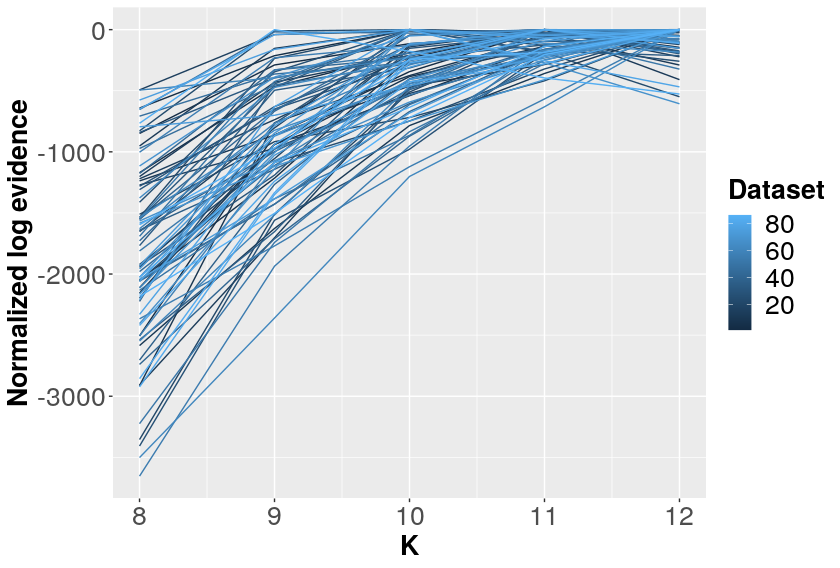
\includegraphics[width=\hsize]{evidence1log}
					\caption{ラプラス近似によって計算されたログエビデンス.各データについて最大値が0となるように定数を足した.}
					\label{fig:evidence1}
			\end{center}
		\end{minipage}
    \begin{minipage}{0.5\hsize}
			\begin{center}
					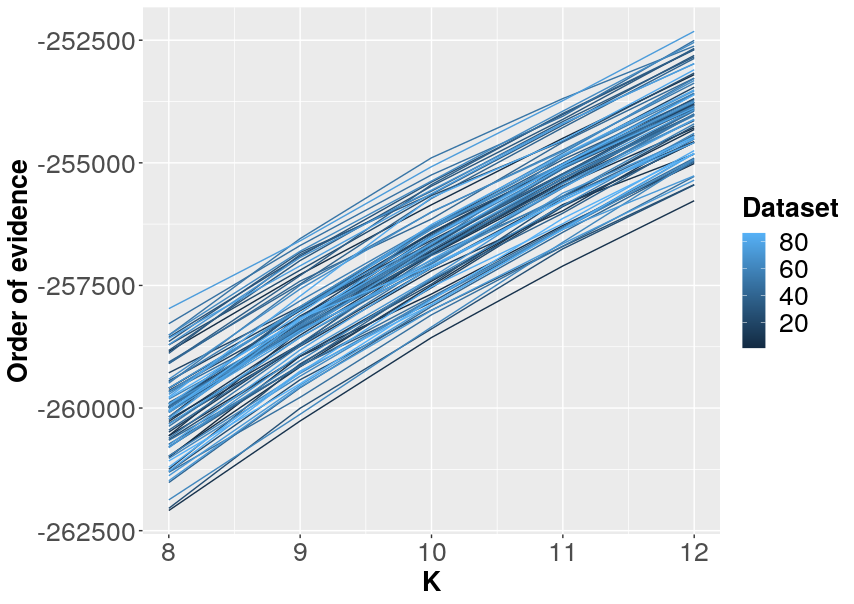
\includegraphics[width=\hsize]{evidence2order}
					\caption{ブートストラップ近似によって計算されたエビデンスのオーダー(10を底とした指数).}
					\label{fig:evidence2}
			\end{center}
		\end{minipage}
\end{figure}

また,\Figref{fig:evidence2}のログを取り,\Figref{fig:evidence1}とプロットした図を\Figref{fig:evidence12}に示す.
これより,ブートストラップによる近似を用いた場合のエビデンスの値は大きいことが分かる.
ラプラス近似では$\frac{d_k}{2} \log n$によって補正された値である.
NMFではデータが増えると補正の値も増えるためラプラス近似は適さないが,\Figref{fig:evidence12}の2つの近似手法のエビデンスの差が過剰に足された補正の値だとも考えることができる.

\begin{figure}[htbp]
    \begin{center}
        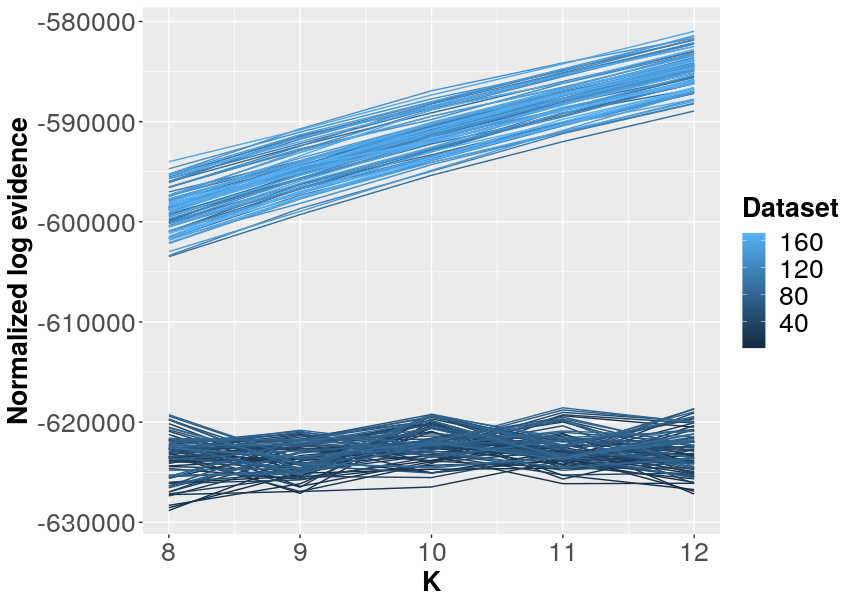
\includegraphics[width=0.8\linewidth]{evidence12log}
        \caption{2つの近似方法によって計算されたログエビデンス.}
        \label{fig:evidence12}
    \end{center}
\end{figure}
